\subsection*{Task 2}

\href{https://github.com/lvjonok/f22-theoretical-mechanics/blob/master/homework5/task2.gif}{simulation}

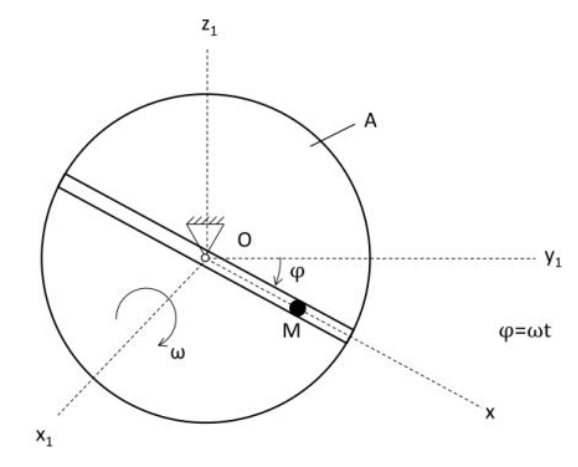
\includegraphics[width=\linewidth]{task2.png}

\begin{enumerate}
    \item RO: particle M - translatory motion, disk A - rotation
    \item Condition:
          \begin{center}
              \begin{tabular}{ |c|c|c| }
                  \hline
                  $$    & $initial$ & $final$ \\
                  \hline
                  $t$   & $0$       & $?$     \\
                  \hline
                  $x$   & $0$       & $r$     \\
                  \hline
                  $x'$  & $0.4$     & $?$     \\
                  \hline
                  $x''$ & $0$       & $0$     \\
                  \hline
              \end{tabular}
          \end{center}
    \item Force analysis: $\vec{G}$, $\vec{N}$
    \item Solution:
          \begin{enumerate}
              \item Equation on x(not static) axis:
                    \begin{align}
                        mx'' = \sum F_x + \Phi_{tr x} + \Phi_{cor x} \\
                        mx'' = mg \sin(\omega t) + m \omega^2 x
                    \end{align}
                    As coriolis acceleration is $\vec{a}_{cor} = 2 (\vec{w}_{tr} \times \vec{v}_{rel})$,
                    we see that its projection on x axis is $0$.
              \item I will not directly solve this equation here,
                    because it just a matter of math (wolfphram)
                    \href{https://www.wolframalpha.com/input?i=y%28t%29%27%27+%3D+g+sin%28wt%29+%2B+w%5E2+y%28t%29%2C+y%280%29%3D0%2C+y%27%280%29%3D0.4}{solution}

                    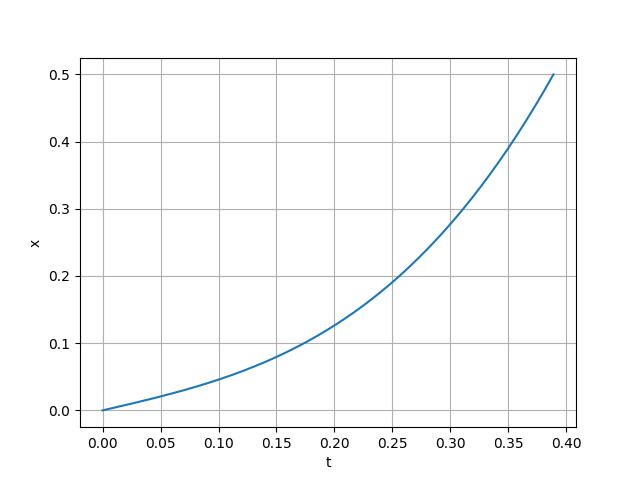
\includegraphics[width=\linewidth]{task2x.png}

              \item At next point we will find $t$ until which we have to simulate everything:
                    \begin{align}
                        x(t) = r
                    \end{align}
              \item Equation on y(not static) axis:
                    \begin{align}
                        ma_{cor} + N - mg \sin(\omega t) = 0 \\
                    \end{align}
                    This equation is enough to find $N$ for each moment of time.

                    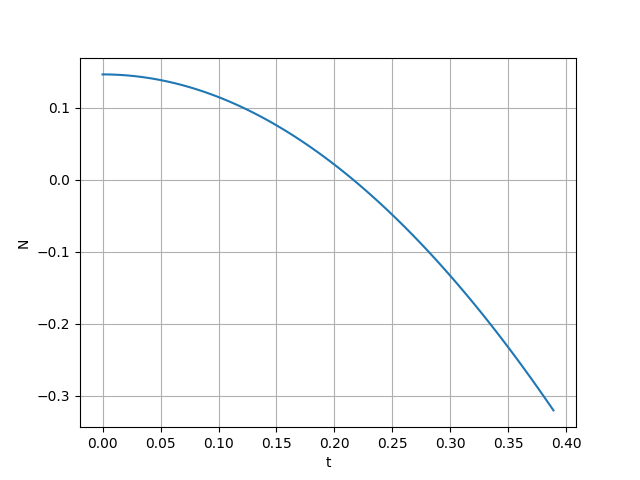
\includegraphics[width=\linewidth]{task2n.png}
          \end{enumerate}
\end{enumerate}

\subsection*{Answer:}

\begin{answer}
    $t_{final} \approx 0.38 s$
\end{answer}